\documentclass[11pt,a4paper]{article}
\usepackage[margin=23mm]{geometry}
\usepackage{fontspec,unicode-math,booktabs,graphicx,array,hyperref}
\setmainfont{STIXGeneral}\setmathfont{STIX Two Math}\hypersetup{hidelinks}
\setlength{\parindent}{0pt}\setlength{\parskip}{5pt}
\newcommand{\tabsetup}{\small\setlength{\tabcolsep}{4pt}\renewcommand{\arraystretch}{1.12}}
\begin{document}
\begin{center}\Large\textbf{Complete papers and shared theories}\\[4pt]
\normalsize Thirteen measured sets, thirty-three original manuscripts\end{center}
This additive overview brings together admitted values. It preserves the earlier 27-original report, adds Matching, Chiral enumeration and the N007 comparison, and uses the enlarged A, B and C editions. The numerical baseline is commit \texttt{c6b1b13}. The subsequent N006 admission is shown separately as \emph{unmeasured}; the old N007 factor does not describe the enlarged orbit-construction topic.

For each topic, $S=\sum_i c(L_i)$ counts the complete originals, $U$ every complete common paper, and $A=\sum_i c(A_i)$ every complete application. The two headline comparisons are
\[
 R=\frac{S}{U+A},\qquad r_i=\frac{c(L_i)}{c(A_i)}
 \quad\text{after acquiring all common theory and declared programs.}
\]
Every topic pays its common theory independently, even when proofs overlap other topics. A factor above one means a shorter replacement in the stated coordinate; a factor below one means a longer replacement. Conditional factors are not standalone application savings.

\textbf{Complete written costs.} All values below are NFC characters excluding whitespace. The fixed whole-document boundaries include their introductions, proofs, local context and references.
\begin{center}\tabsetup\begin{tabular}{lrrrrrr}\toprule
Topic & Originals & Sources & Common & Applications & Written & Factor\\\midrule
A & 7 & 213,803 & 49,059 & 87,019 & 136,078 & 1.571 \\
B & 5 & 124,906 & 42,547 & 76,243 & 118,790 & 1.051 \\
C & 5 & 118,433 & 30,437 & 61,248 & 91,685 & 1.292 \\
D & 3 & 47,894 & 15,632 & 29,855 & 45,487 & 1.053 \\
E & 3 & 71,375 & 19,790 & 19,513 & 39,303 & 1.816 \\
F & 1 & 25,115 & 7,118 & 12,744 & 19,862 & 1.264 \\
G & 2 & 73,199 & 30,928 & 85,207 & 116,135 & 0.630 \\
Affine & 1 & 32,767 & 19,070 & 22,638 & 41,708 & 0.786 \\
Represent. & 1 & 25,348 & 11,288 & 13,688 & 24,976 & 1.015 \\
Chamber & 2 & 35,802 & 15,199 & 21,254 & 36,453 & 0.982 \\
Matching & 1 & 37,951 & 16,732 & 17,168 & 33,900 & 1.119 \\
Chiral & 1 & 29,599 & 8,831 & 23,171 & 32,002 & 0.925 \\
Diagonal* & 1 & 22,888 & 10,968 & 11,771 & 22,739 & 1.007 \\
\bottomrule\end{tabular}\end{center}
\textbf{Representations remain distinct.} B and C use complete authored text renderings for N001 and L108; all other source and replacement PDFs in those two topics are counted raw and untrimmed. Their older original-PDF coordinates remain unknown. The other rows use accepted calibrated, selected PDF text with exact repeated furniture removed. No pooled factor across these representations is formed.

\textbf{Scope.} These are 33 measured originals within the fixed 161-item programme. The current scientific register has 34 admitted recoveries among 104 accessible originals, with N006 awaiting measurement; 70 accessible originals await complete recovery and 57 remain retrieval targets. Complete numerators match the declared principal-result contracts, with corrections, retained facts and ancillary exclusions preserved. This report changes no scientific, question or formal credit.
\newpage
\textbf{Full common theories and applications.}
Each row has one scale for its original sum and replacement. Blue segments are whole common papers; green segments are individual complete applications. B pays both common papers (14,124 and 28,423). C pays its original common paper (27,142) and the entire incidence note (3,295). All segments remain charged.
\begin{center}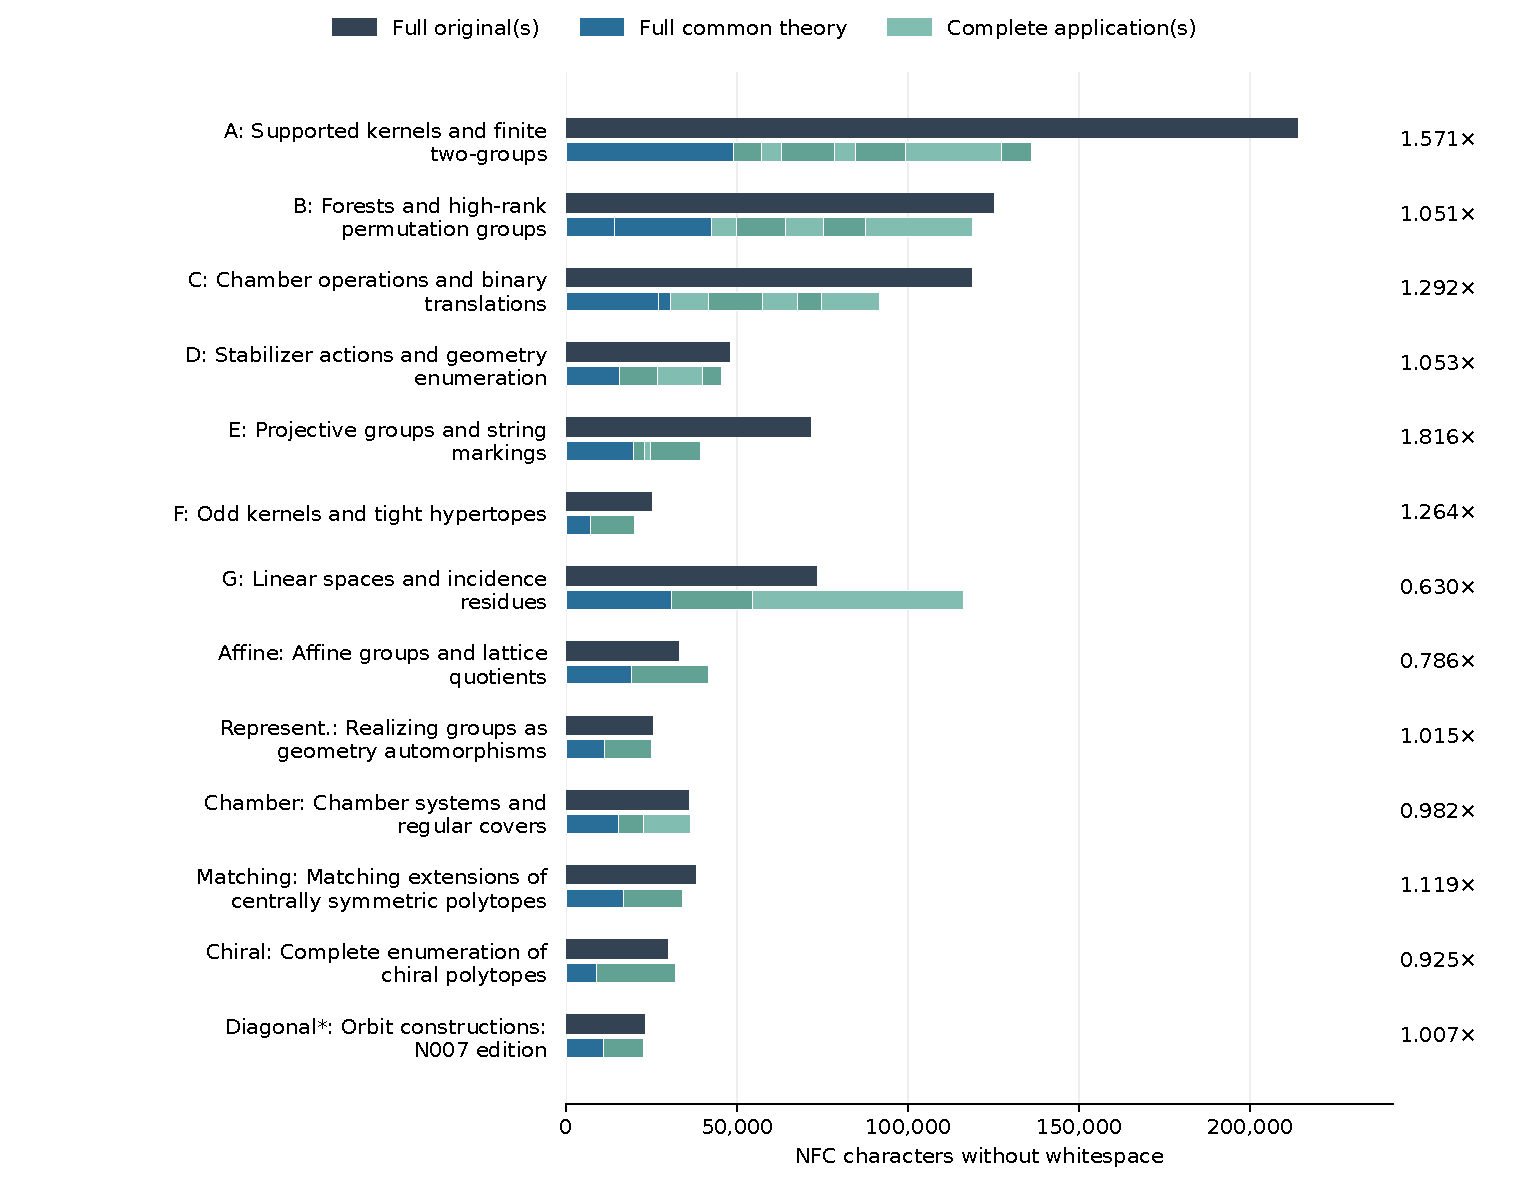
\includegraphics[width=\linewidth]{whole_topics.pdf}\end{center}
The Diagonal row concerns only the earlier N007 edition. There is no bar or numerical placeholder for N006, and no measured whole-topic factor for the expanded N006+N007 edition. Text length is not a minimum proof complexity or a measure of mathematical originality.
\newpage
\textbf{Complete programs and prior acquisition.}
The written comparison remains first. These separate alternatives add the entire declared printed appendix, or its entire raw program files, to the written denominator. Printed and raw code are never added together.
\begin{center}\tabsetup\begin{tabular}{lrrrrr}\toprule
Topic & Printed code & With printed & Raw code & With raw & $U+$printed\\\midrule
A & 54,210 & 1.124 & 52,807 & 1.132 & 103,269 \\
B & 13,170 & 0.947 & 12,330 & 0.953 & 55,717 \\
C & 20,933 & 1.052 & 19,937 & 1.061 & 51,370 \\
D & 27,070 & 0.660 & 26,185 & 0.668 & 42,702 \\
E & 7,565 & 1.523 & -- & -- & 27,355 \\
F & 8,837 & 0.875 & 8,061 & 0.899 & 15,955 \\
G & 53,018 & 0.433 & 50,184 & 0.440 & 83,946 \\
Affine & 17,250 & 0.556 & 16,682 & 0.561 & 36,320 \\
Represent. & 9,025 & 0.746 & 8,310 & 0.762 & 20,313 \\
Chamber & 7,677 & 0.811 & 6,401 & 0.835 & 22,876 \\
Matching & 4,998 & 0.976 & 4,408 & 0.991 & 21,730 \\
Chiral & 11,940 & 0.674 & 11,090 & 0.687 & 20,771 \\
Diagonal* & 3,161 & 0.884 & 2,856 & 0.894 & 14,129 \\
\bottomrule\end{tabular}\end{center}
The final column is prepaid in every conditional row for that topic. E preserves its admitted convention: its optional validation program costs another 5,173 characters and gives a separate program-inclusive factor of 1.372. An unadmitted raw-code alternative for E is not invented here.

\textbf{Program roles.} A includes all five files. B includes one finite proof premise, two validations and an auxiliary example. C includes its three complete GAP files; the identical shared construction is charged once, and its exhaustive census remains paid. D includes five required and three diagnostic programs. E separates one required program from optional validation. F's three programs and Representation's two are validations, not uniform proof premises. G retains four finite computations, two certificate bridges and seven validations. Affine retains all six mathematical programs. Chamber retains one required GAP program and one diagnostic. Matching's census is a finite premise. Chiral enumeration retains all three enumeration/formula/validation programs. The N007 edition includes its whole validation program. Separate operational drivers and partial Lean inventories stay separate, as in the admitted packets.

\textbf{Limits.} Retained full external proofs, unprovided historical software, complete graphic information and end-to-end formalization have unknown costs, not zero. Units matter: Representation's written factor is about 0.971 in its admitted UTF-8 coordinate, and Chiral enumeration is about 1.003 in whitespace tokens but 0.925 in nonspace characters. All underlying multi-unit sensitivities remain available; this table consistently uses the declared primary character coordinate.
\newpage
\textbf{Every complete application after full acquisition.}
All common papers and all declared programs in the preceding table have already been paid. The source and application are complete documents under the same topic boundary; no smaller theorem closure replaces either side.
\begin{center}\tabsetup\begin{tabular}{lllrrr}\toprule
Topic & Original & Application & Source cost & Application cost & Conditional\\\midrule
A & L032 & A1 & 16,558 & 8,212 & 2.016 \\
A & L034 & A2 & 21,433 & 5,784 & 3.706 \\
A & F016 & A3 & 43,983 & 15,419 & 2.853 \\
A & F013 & A4 & 25,562 & 6,224 & 4.107 \\
A & L035 & A5 & 51,019 & 14,498 & 3.519 \\
A & N009 & A6 & 36,824 & 28,114 & 1.310 \\
A & L128 & A7 & 18,424 & 8,768 & 2.101 \\
B & N001 & B1 & 14,519 & 7,371 & 1.970 \\
B & N003 & B2 & 17,780 & 14,170 & 1.255 \\
B & N008 & B3 & 18,009 & 11,132 & 1.618 \\
B & L030 & B4 & 22,704 & 12,286 & 1.848 \\
B & L040 & B5 & 51,894 & 31,284 & 1.659 \\
C & L088 & C1 & 13,166 & 11,311 & 1.164 \\
C & N013 & C2 & 27,361 & 15,815 & 1.730 \\
C & L108 & C3 & 12,849 & 10,075 & 1.275 \\
C & F014 & C4 & 20,577 & 6,962 & 2.956 \\
C & L068 & C5 & 44,480 & 17,085 & 2.603 \\
D & L066 & D1 & 20,916 & 10,989 & 1.903 \\
D & L074 & D2 & 20,661 & 13,367 & 1.546 \\
D & L104 & D3 & 6,317 & 5,499 & 1.149 \\
E & L083 & E1 & 20,885 & 3,002 & 6.957 \\
E & L079 & E2 & 20,908 & 1,855 & 11.271 \\
E & L021 & E3 & 29,582 & 14,656 & 2.018 \\
F & L014 & F1 & 25,115 & 12,744 & 1.971 \\
G & L009 & G1 & 49,891 & 23,544 & 2.119 \\
G & L092 & G2 & 23,308 & 61,663 & 0.378 \\
Affine & L012 & AF1 & 32,767 & 22,638 & 1.447 \\
Represent. & F010 & R1 & 25,348 & 13,688 & 1.852 \\
Chamber & L008 & H1 & 21,784 & 7,571 & 2.877 \\
Chamber & N016 & H2 & 14,018 & 13,683 & 1.024 \\
Matching & F015 & M1 & 37,951 & 17,168 & 2.211 \\
Chiral & L028 & CE1 & 29,599 & 23,171 & 1.277 \\
Diagonal* & N007 & DG1 & 22,888 & 11,771 & 1.944 \\
\bottomrule\end{tabular}\end{center}
The asterisk on Diagonal identifies the earlier N007-only acquisition. These individual factors cannot be transferred to a new common edition without a newly fixed measurement. No node-count factor is used.
\newpage
\textbf{Individual source and application costs: first seventeen originals.}
Dark bars show complete originals; green bars show their complete applications. Factors at right assume full prior acquisition, including the enlarged B and C common theory and all declared programs. A shared scale is used within this chart.
\begin{center}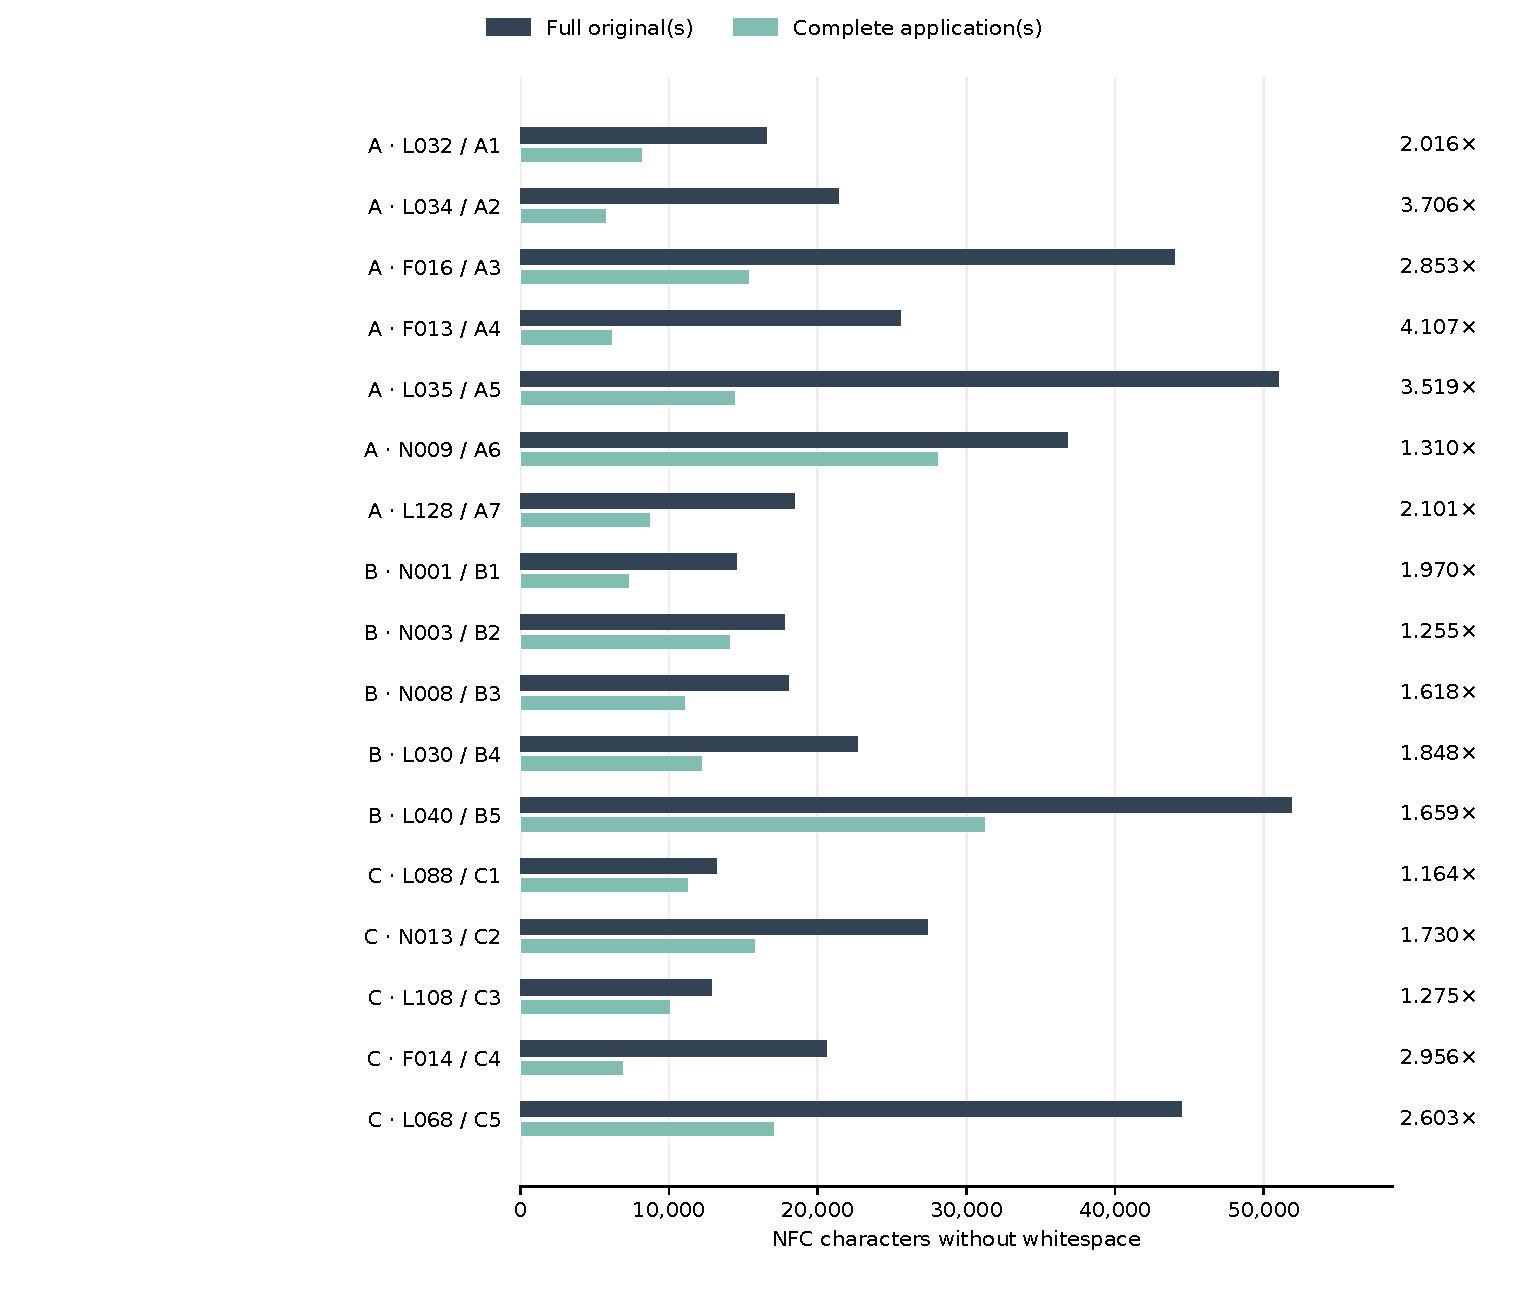
\includegraphics[width=\linewidth]{conditional_1.pdf}\end{center}
Source IDs are stable catalogue labels. Their exact definitions, source editions and proof contracts remain in the linked admitted measurements; they are not additional mathematical claims of this overview.
\newpage
\textbf{Individual source and application costs: remaining sixteen originals.}
The same conventions apply; the scale is shared by every source/application pair in this chart. No cost for N006 is inferred from the last row.
\begin{center}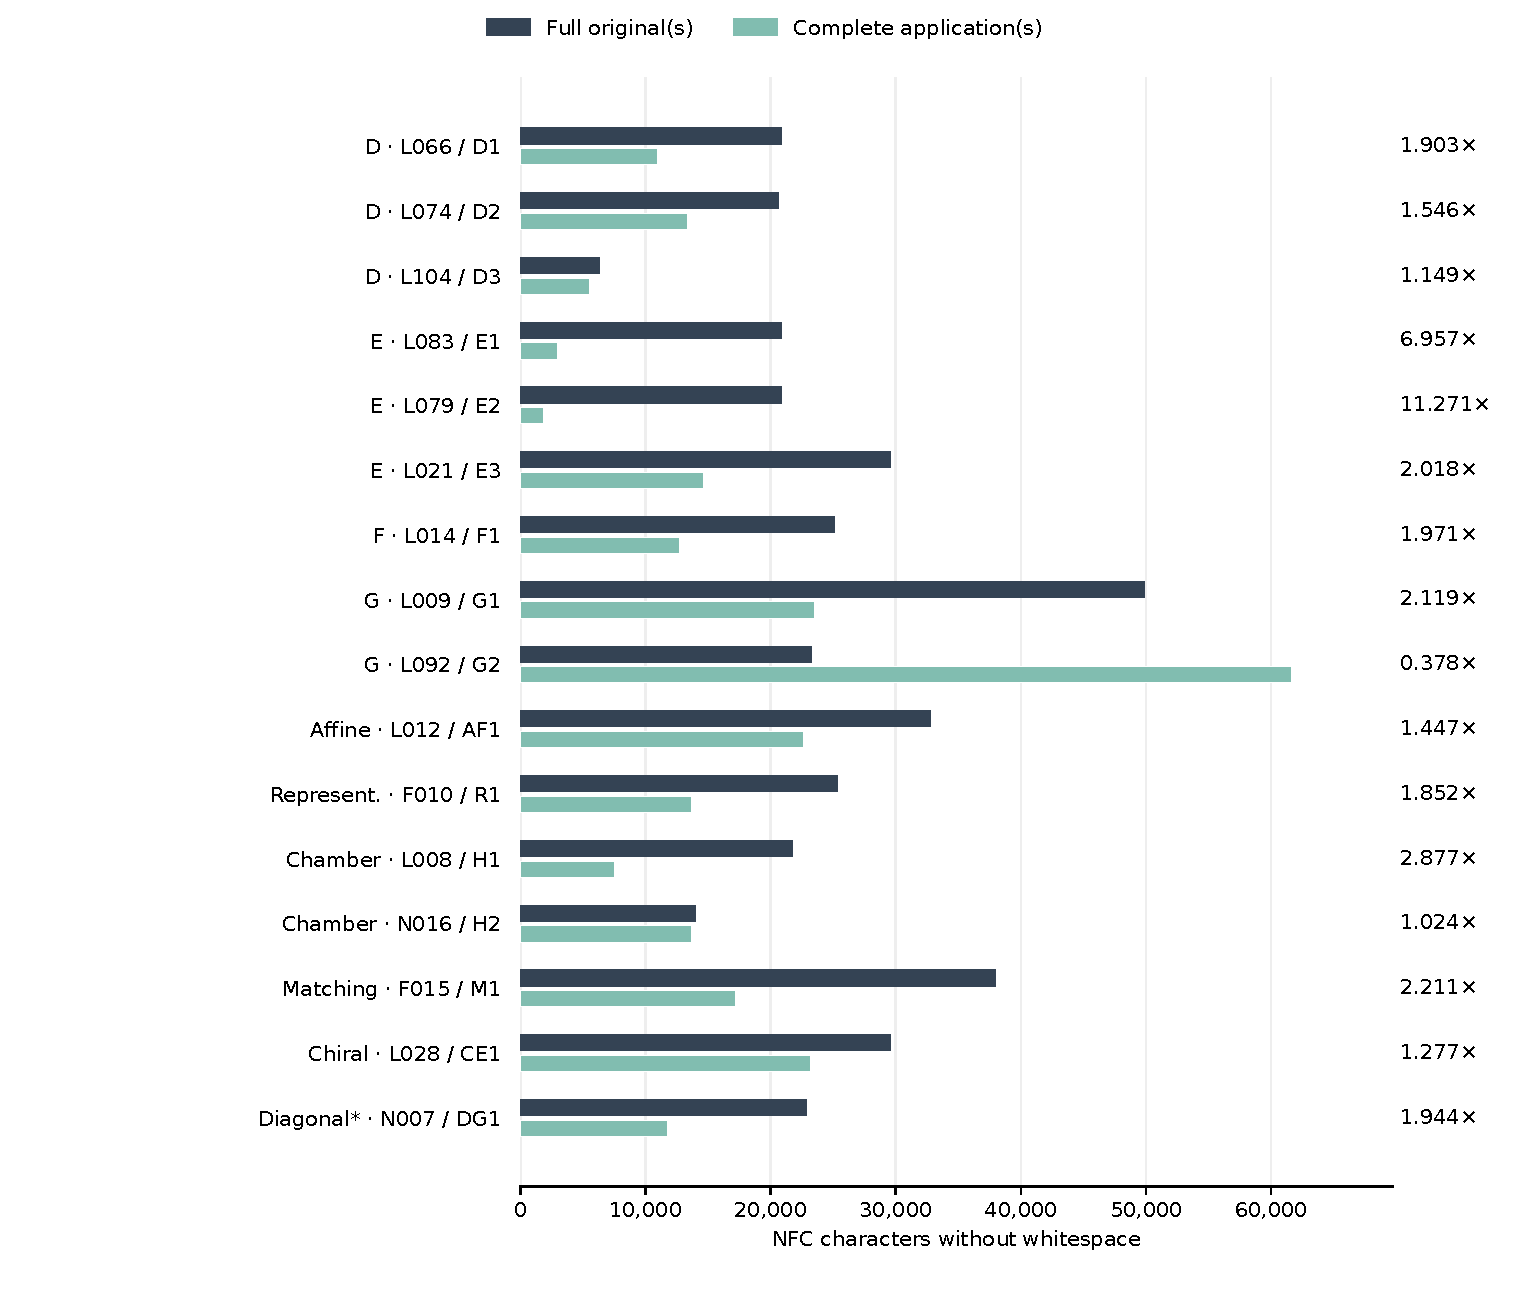
\includegraphics[width=\linewidth]{conditional_2.pdf}\end{center}
\textbf{Exact data and provenance.} The accompanying \texttt{results.json}, \texttt{topics.csv} and \texttt{applications.csv} retain exact integer costs and rational factors. \texttt{protocol.json} pins the old admitted overview, four admitted numerical updates, their independent records and the unmeasured N006 admission. No primary text was copied or extracted in this consolidation. Graph bars use these same costs; they do not depict theorem counts or claims of optimality. The new consolidation requires distinct review before publication.
\end{document}
